\section{Benchmark NIST-3 "Linear Elasticity"}
\label{sec:bench-3}

This is a system of two coupled equations with a mixed
derivative for linear elasticity in the coupling term.
This example employs the adaptive multimesh $hp$-FEM 
to solve equations of linear elasticity.

\begin{equation} \label{crack-u}
-E \frac{1-\nu^2}{1-2\nu} \frac{\partial^{2} u}{\partial x^{2}} - E\frac{1-\nu^2}{2-2 \nu} \frac{\partial^{2} u}{\partial y^{2}}
-E \frac{1-\nu^2}{(1-2\nu)(2-2\nu)} \frac{\partial^{2} v}{\partial x \partial y} = F_{x}
\end{equation}
\begin{equation} \label{crack-v}
-E \frac{1-\nu^2}{2-2\nu} \frac{\partial^{2} v}{\partial x^{2}} - E\frac{1-\nu^2}{1-2\nu} \frac{\partial^{2} v}{\partial y^{2}}
-E \frac{1-\nu^2}{(1-2\nu)(2-2\nu)} \frac{\partial^{2} u}{\partial x \partial y} = F_{y},
\end{equation}
where $F_{x} = F_{y} = 0$, $u$ and $v$ are the
$x$ and $y$ displacements, $E$ is Young's Modulus,
and $\nu$ is Poisson's ratio.

The domain is $\Omega = (0, 1)^2$, equipped with Dirichlet
boundary conditions given by the exact solution.

The exact solution:
\begin{equation}\label{exact-nist-3-u-1}
u(x, y) = \frac{1}{2G} r^{\lambda}[(k - Q(\lambda + 1))cos(\lambda \theta) - \lambda cos((\lambda - 2) \theta)]
\end{equation}
\begin{equation}\label{exact-nist-3-v-1}
v(x, y) = \frac{1}{2G} r^{\lambda}[(k + Q(\lambda + 1))sin(\lambda \theta) + \lambda sin((\lambda - 2) \theta)]
\end{equation}
here $\lambda = 0.5444837367825$, $Q = 0.5430755788367$,
$k = 3 - 4 \nu$ and $G = E / (2(1 + \nu))$.

The solution of NIST-3 is shown in Fig. \ref{fig:sln-nist03}.

\begin{figure}[!ht]
\centering
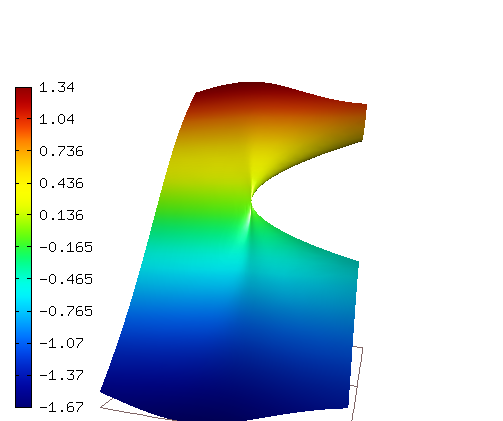
\includegraphics[height=50mm]{nist/nist-3/solution-u.png}\ \
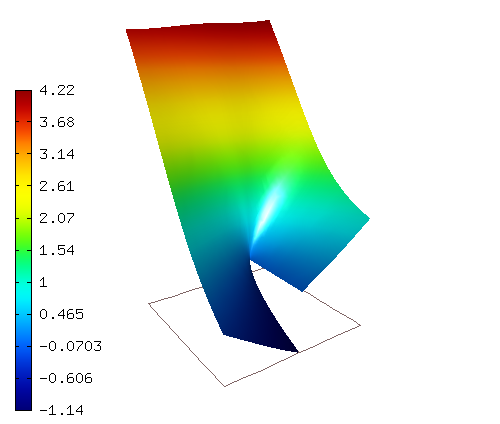
\includegraphics[height=50mm]{nist/nist-3/solution-v.png}
\vspace{-2mm}
\caption{The $u$ and $v$ component to NIST-3 benchmark problem.}
\label{fig:sln-nist03}
\end{figure}
